\section{Evaluation} \label{sec:eval}

\begin{table}[t]
\begin{center}
\begin{tabular}{|c|c|c|c|c|c|}\hline
& & \multicolumn{2}{|c|}{original} & \multicolumn{2}{|c|}{incremental} \\ \cline{3-6}
\raisebox{1.5ex}[0pt]{Formats} & \raisebox{1.5ex}[0pt]{k Lines/KB} & 
	Time & TC & Time & TC \\ \hline \hline
interface & 1.2/185		& 48.5	& 0.7	& 2.9	& 1.1 \\ \hline
asl.log  &	1.5/552		& 31.9	& 0.9	& 13.5 	& 1.5 \\ \hline
%apache.txt  &	2087&442	& 66.4 & 1746.1 & 7.9 	& 2277.6 \\ \hline
%ai.3000	&	3000&286	& 26	& 412.6	& 2.2	& 440.6	\\ \hline
error\_log  &	4.5/409		& 93.1	& 0.1	& 0.9	& 0.1 \\ \hline
access\_log  &	8.2/551 	& 130.5	& 0.3	& 2.8	& 0.3	\\ \hline
coblitz	     & 9.4/2561   	& -	& -	& 31.9 & 2.9 \\ \hline
pws	&	 17.4/3432	& -	& - 	& 133  & 5.7 \\ \hline
ai.big	&	57.4/5608	& -	& -	& 26.2	& 543 \\ \hline
exlog & 260.8/76720 		& -	& -	& 610 & 3.0 \\ \hline
redirect & 302.6/102404 	& -	& -	& 1852 & 17.1 \\ \hline
getbig & 550.4/92192   		& -	& -	& 668 & 8.8 \\ \hline
\end{tabular}
\caption{Exec. times (secs) and Type Complexities (kb)} 
\label{tab:results}
\end{center}
\end{table}

The first experiment was conducted on a PowerBook G4 with a 1.67GHz PowerPC
CPU and 2G memory running on Mac OS X 10.4. 
Table \ref{tab:results} compares the performance results between
the original \learnpads{} system and the incremental system. 
The benchmarks used are 10 system logs with various sizes. 
Column 2 shows the number of lines and the KB size of each log. 
The time columns record the total
running time in seconds, and the $TC$ columns record the type complexity
of the final description learned. Intuitively, the type complexity
is the cost of transmitting (in bits) the sort of description (\ie{}, \cd{struct},
\cd{union}, \cd{enum}, \etc{}) plus the cost of transmitting all of its
subcomponents. In general, lower type complexity means
more compact description. For all benchmarks, the initial learn size $N$ is 500 lines 
and the incremental learn size $M$ is 100 lines. 
The slight twist is that the initial learn chunk is not the first $N$ lines in the
data, but a mix of the $N/3$ consecutive lines taken from the beginning, middle,
and end of the data source. 
Where it takes more than half an hour for the original \learnpads{}
system to learn a description, a ``-'' is put in those cells to 
indicate there is no result. Table \ref{tab:results} shows that
the incremental algorithm learns a description slightly less compact than the
original algorithm but in much shorter time. We also verified the correctness of the learned
description by running an accumulator tool \cite{fisher+:pads} generated from the 
description on the original data to see if there is any parsing errors. 
It turns out that all data sources can be correctly parsed for pws which 
is a web server log produced by the Apache web server. 
The parsing errors were caused by the way union branches are ordered in the learned 
description. We are exploring a different
\pads{} backend that would resolve this problem.

\begin{figure}[t]
\begin{center}
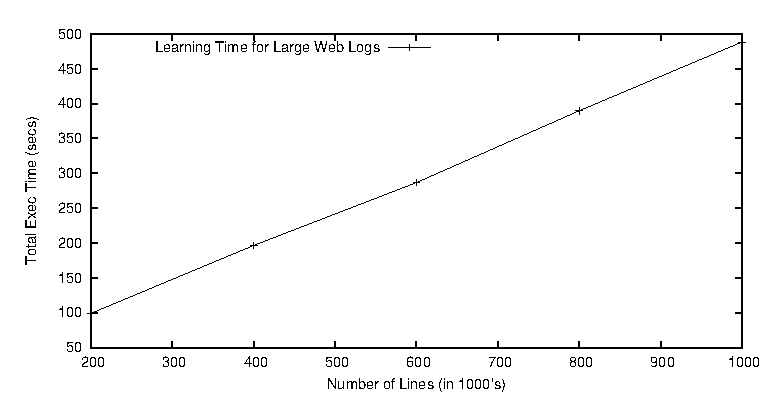
\epsfig{file=scale.eps,width=0.9\columnwidth}
\caption{Scaling of increment algorithm}
\label{fig:scale}
\end{center}
\end{figure}

The second experiment measures the execution time of learning 
a series of large web logs ranging from 200k lines to 1 million lines. Because
these data sources are private to AT\&T, the experiment was run on 
an AT\&T internal server which is ... ...
Figure \ref{fig:scale} shows our algorithm scales almost linearly with the size
of the data. In particular, the algorithm learns a description from a million-line
web log in under 10 minutes.

% - parse metric
% - initial learn size and chunk size - these can affect results
% - update chunk by chunk 
% - optimizations/heuristics
%   due to performance concerns:
%   - memoization
%   - the clean function (to reduce the number of parses)
%   - control of aggregate size
%   - parses cut-off: kill a parse if it has more than n consecutive failures in a struct
%   due to quality of description concerns (and also performance)
%   - deterministic unions
%   - longest match in arrays
%   - merge adjacent const strings (only punctuation and white spaces)
%   - error recovery
%
%- Experiments
%	1) comparison with old LearnPADS on several large datasets (ai.3000, asl.log, apache.txt, access\_log, error\_log, interface.loop)
%	   compare exec time and type complexity. For increment, use
%	   initial learn chunk of 100 and incremental error chunks of 100
%	2) use ai format, do a table with 1000 5000 10000,...,1M miles
%	   using orig learning system and the new system with various optimization turned on and off.
%

